% =========================================================================
\chapter{Generative models}
\label{ch:gen}
% =========================================================================

\section{Neural network basics (just enough)}
A \textbf{neuron} multiplies each input $x_i$ by a weight $w_i$, adds them and a bias $b$, and passes the sum through
an \textbf{activation function} $f$ such as ReLU ($\max(0,z)$) or SiLU (a smooth version):
$\hat y=f(w_1x_1+\dots+w_nx_n+b)$. A \textbf{layer} is many neurons side by side; a \textbf{network} is layers in a row
(``$128\to128$'' means two layers of 128 neurons).

\begin{figure}[H]
\centering
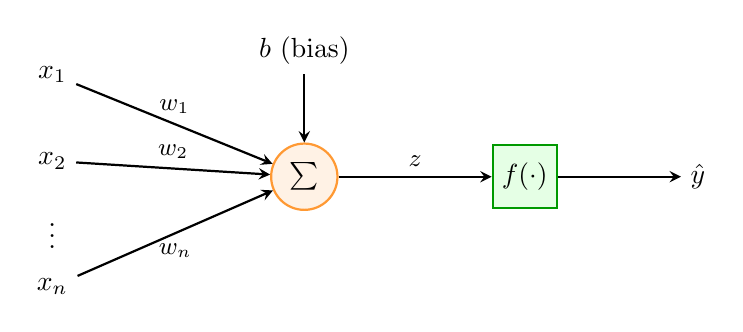
\begin{tikzpicture}[
  neuron/.style={circle,draw=blue!80,fill=blue!10,thick,minimum size=8mm},
  sum/.style={circle,draw=orange!80,fill=orange!10,thick,minimum size=8mm},
  act/.style={rectangle,draw=green!60!black,fill=green!10,thick,minimum size=8mm},
  arrow/.style={->,>=stealth,thick}]
\node (x1) at (0,1.6) {$x_1$}; \node (x2) at (0,0.5) {$x_2$}; \node at (0,-0.35) {$\vdots$}; \node (xn) at (0,-1.1) {$x_n$};
\node[sum] (s) at (3.2,0.3) {$\sum$}; \node[act] (f) at (6,0.3) {$f(\cdot)$}; \node (y) at (8.2,0.3) {$\hat y$};
\draw[arrow] (x1) -- node[above,font=\small]{$w_1$} (s); \draw[arrow] (x2) -- node[above,font=\small]{$w_2$} (s);
\draw[arrow] (xn) -- node[below,font=\small]{$w_n$} (s);
\node (b) at (3.2,1.9) {$b$ (bias)}; \draw[arrow] (b) -- (s);
\draw[arrow] (s) -- node[above,font=\small]{$z$} (f); \draw[arrow] (f) -- (y);
\end{tikzpicture}
\caption{One artificial neuron.}
\end{figure}

\textbf{Training} repeats three steps: (1) \emph{forward pass}: compute outputs and a \textbf{loss} (how wrong they
are); (2) \emph{backpropagation}: compute how the loss changes with every weight (the gradient); (3) \emph{update}: move
each weight a small step against its gradient (gradient descent; \textbf{Adam} and \textbf{AdamW} are popular versions
that adapt the step size). A \textbf{batch} is the number of rows used for one update; an \textbf{epoch} is one pass
over all training rows; the \textbf{learning rate} is the step size.

\section{What a generative model is}
A classifier learns to \emph{answer} (is this day extreme?). A \textbf{generative model} learns the \emph{shape of the
data} so it can \emph{produce new, realistic examples}. Here each generator learns from the 29{,}604 real extreme rows of
the training years and then produces new extreme rows: 49 numbers (the predictor groups A--D) plus the season. The 8
gap-to-threshold numbers (group E) are always recomputed afterwards. All three generators are trained from scratch.

\section{TVAE: a variational autoencoder}
\begin{figure}[H]
\centering
\begin{tikzpicture}[node distance=4mm]
\node[bdat,text width=1.7cm] (x) {real day\\49 + season};
\node[bx,text width=1.7cm,right=of x] (t) {mode split\\(prepare)};
\node[orange box,text width=1.7cm,right=of t] (e) {encoder\\$128\to128$};
\node[blue box,text width=1.7cm,right=of e] (h) {code\\128 numbers};
\node[orange box,text width=1.7cm,right=of h] (d) {decoder\\$128\to128$};
\node[bdat,text width=1.7cm,right=of d] (y) {rebuilt day};
\foreach \a/\b in {x/t,t/e,e/h,h/d,d/y} \draw[ar] (\a) -- (\b);
\node[bdat,text width=3.6cm,below=7mm of h] (n) {new day: random code $\rightarrow$ decoder};
\draw[ar,dashed] (n.east) -| (d.south);
\end{tikzpicture}
\caption{TVAE (Xu et al., NeurIPS 2019).}
\end{figure}
\begin{itemize}
  \item \textbf{Autoencoder:} the \emph{encoder} squeezes a day into a short \textbf{code} (also called the latent
        vector), the \emph{decoder} rebuilds the day from it. Learning to rebuild forces the code to capture what
        matters.
  \item \textbf{Variational:} the code is drawn from a bell curve with a learned mean $\mu$ and spread $\sigma$
        ($\mathbf h=\mu+\sigma\epsilon$, the \emph{reparameterisation trick}), and a \textbf{KL term} in the loss keeps
        all codes close to a standard bell curve. Then \emph{any} random code from that bell curve decodes to a
        sensible day: that is how new days are made.
  \item \textbf{Loss (ELBO):} rebuild error + KL term.
  \item \textbf{Tabular (``T''):} each number column is first split into its typical ranges (\emph{modes}) using a
        Gaussian mixture, so skewed columns such as rain are handled well.
  \item \textbf{Weakness:} rebuilding rewards typical rows, so it tends to average: its extremes are mostly mild. 75\%
        of its raw rows broke a physical rule before clean-up.
  \item \textbf{Settings:} code of 128, encoder and decoder of two layers of 128 (library defaults), 300 epochs,
        batch 500.
\end{itemize}

\section{CTGAN: a conditional generative adversarial network}
\begin{figure}[H]
\centering
\begin{tikzpicture}[node distance=5mm]
\node[bdat,text width=2.0cm] (z) {noise (128)\\+ a season};
\node[orange box,text width=2.2cm,right=of z] (g) {generator\\2 residual layers\\of 256};
\node[blue box,text width=1.6cm,right=of g] (f) {fake day};
\node[orange box,text width=2.2cm,right=of f] (c) {critic\\$256\to256$\\sees 10 days};
\node[bdat,text width=1.6cm,right=of c] (s) {real or\\fake?};
\node[bdat,text width=2.4cm,below=7mm of c] (r) {real extreme days};
\foreach \a/\b in {z/g,g/f,f/c,c/s} \draw[ar] (\a) -- (\b);
\draw[ar] (r) -- (c);
\end{tikzpicture}
\caption{CTGAN (Xu et al., NeurIPS 2019).}
\end{figure}
\begin{itemize}
  \item \textbf{Two networks that compete:} the \emph{generator} turns random noise into a fake day; the \emph{critic}
        (discriminator) tries to tell fake days from real ones. Each improves against the other until fake days look
        real. Like a forger and a detective.
  \item \textbf{Conditional:} the generator is also given a season, and must produce a day of that season.
        \emph{Training-by-sampling} shows rare seasons often enough that they are learned.
  \item \textbf{WGAN-GP loss:} the critic gives a realness score rather than a yes/no, and a \emph{gradient penalty}
        keeps it smooth. This makes training more stable than the original GAN.
  \item \textbf{Packing (pac 10):} the critic judges 10 days together, so the generator cannot fool it by repeating one
        good day (\emph{mode collapse}).
  \item \textbf{Weakness:} it learns to fool the critic, not physics: 69\% of raw rows broke a rule. Strength: it
        reached the hot tail best on its own.
  \item \textbf{Settings:} noise of 128, generator and critic of two layers of 256 (library defaults), 300 epochs,
        batch 500, learning rate $2\times10^{-4}$.
\end{itemize}

\section{Conditional diffusion model (DDPM)}
\begin{figure}[H]
\centering
\begin{tikzpicture}[x=1.55cm]
\foreach \i/\l/\c in {0/real day/black!4,1/a little noise/black!10,2/more noise/black!18,3/\dots/white,4/pure noise/black!30}
  \node[bx,fill=\c,text width=1.3cm] (n\i) at (\i*1.6,0) {\l};
\foreach \i in {0,...,3} { \pgfmathtruncatemacro{\j}{\i+1}
  \draw[ar,black!50] ([yshift=2mm]n\i.east) -- ([yshift=2mm]n\j.west);
  \draw[ar,orange!70!black] ([yshift=-2mm]n\j.west) -- ([yshift=-2mm]n\i.east); }
\node[font=\scriptsize,black!60,anchor=south] at (3.2,0.55) {training: add noise step by step (1,000 steps)};
\node[font=\scriptsize,orange!70!black,anchor=north] at (3.2,-0.55) {generating: remove noise step by step (50 steps), guided by season and severity};
\end{tikzpicture}
\caption{The idea of diffusion (Ho et al., NeurIPS 2020).}
\end{figure}
\begin{itemize}
  \item \textbf{Forward process (training):} take a real day and add a little random noise, again and again, over
        1{,}000 steps, until nothing is left but noise. The amount added at each step follows a \emph{cosine
        schedule}.
  \item \textbf{What the network learns:} given a noisy day, how noisy it is (the step $t$), and the condition (season
        and severity $z$), guess the noise that was added. Loss = squared error of that guess.
  \item \textbf{Reverse process (generating):} start from pure noise and remove the guessed noise step by step. Using
        the \textbf{DDIM} shortcut, 50 steps are enough instead of 1{,}000.
  \item \textbf{Classifier-free guidance:} in training the condition is hidden 10\% of the time, so the same network
        can guess the noise with and without it. When generating, the two guesses are combined,
        $\tilde\epsilon=(1+w)\,\epsilon(\text{with condition})-w\,\epsilon(\text{without})$, with $w=2$: this pushes
        the day towards the requested season and severity.
  \item \textbf{Network:} the noisy day, the step and the condition are each turned into 512 numbers and added; four
        \emph{residual blocks} (each: normalise, widen to 1{,}024, SiLU, back to 512, and add its input back) predict
        the noise. About 4.85 million weights. Inputs are first mapped to a bell curve (quantile transform).
  \item \textbf{Training:} AdamW, learning rate $10^{-3}$, 15{,}000 steps of 1{,}024 rows, and an averaged copy of the
        weights (EMA 0.999) used for generating.
  \item \textbf{Strengths:} can be \emph{asked} for an exact season and severity (the only one of the three); almost no
        raw rows broke physics; its days were the closest to real ones.
\end{itemize}

\section{From generator to training data}
\begin{figure}[H]
\centering
\begin{tikzpicture}[node distance=4mm]
\node[bdat,text width=2.0cm] (a) {29{,}604\\real extreme\\rows};
\node[orange box,text width=2.0cm,right=of a] (b) {generator\\trained\\from scratch};
\node[orange box,text width=2.0cm,right=of b] (c) {296{,}040\\raw rows\\($10\times$)};
\node[red box,text width=2.0cm,right=of c] (d) {clean-up +\\EVT selection:\\88{,}812 ($3\times$)};
\node[green box,text width=2.0cm,right=of d] (e) {29{,}604 added\\to one\\training run};
\foreach \u/\v in {a/b,b/c,c/d,d/e} \draw[ar] (\u) -- (\v);
\end{tikzpicture}
\caption{Counts for TVAE and CTGAN. The diffusion model is asked directly for the EVT severities.}
\end{figure}
\begin{itemize}
  \item \textbf{Consistency clean-up} (the code calls it ``physics''; say ``consistency and range clean-up''):
        each generated row is moved to the nearest real cell (taking its real height and slope); the three daily
        temperatures are \emph{sorted} so that minimum $\le$ mean $\le$ maximum; dewpoint is capped at the mean
        temperature; humidity is cut to 0--100\%; rain and sunshine are cut at 0; soil water is cut to 0--0.8; counts
        are cut to range and rounded; the 8 gap columns are recomputed from that cell's threshold. It removes
        impossible values; it does \emph{not} make a day realistic (see the box below).
  \item \textbf{Judge model (TVAE and CTGAN only):} these two cannot be asked for a severity, so a separate LightGBM
        model, trained on real extremes, estimates the severity $z$ of each generated row; rows are then picked so that
        their tail positions match the EVT target (60\% in the top fifth) and their seasons match the real shares.
  \item \textbf{Placement:} the season follows the share of real extremes per season; the location is generated with
        the day and snapped to a real cell; so new days appear where extremes really occur.
\end{itemize}


\begin{keyidea}[What the clean-up does not do (say it before they ask)]
\begin{itemize}
  \item Humidity is not recomputed after the dewpoint is capped, so humidity, temperature and dewpoint can disagree.
  \item Temperature is not checked against the height of the cell the row is snapped to (a 40\,$^\circ$C row can land
        on a 4{,}000\,m cell; its gap columns then become very large).
  \item Anomaly and 7--30-day history columns are not recomputed from the daily values.
\end{itemize}
Real data break none of the rules (about 0\%); raw TVAE rows broke at least one in 75\% of cases, CTGAN in 69\%, the
diffusion model in about 0\%.
\end{keyidea}

\begin{keyidea}[Why 0.8 for soil moisture?]
\textbf{What the number is.} Soil moisture here (\texttt{swvl1}) is \emph{volumetric}: the fraction of the top 7\,cm
of soil that is water, in m$^3$\,m$^{-3}$. It can never be larger than the share of the soil that is empty space
(its \emph{saturation} or porosity): once every pore is full, no more water fits.

\textbf{What ERA5-Land allows.} ERA5-Land's land model (H-TESSEL) gives each soil texture a saturation value taken
from the European HYPRES soil table: about 0.40 for coarse (sandy) soil and at most 0.766 for organic soil. So the
model itself can never produce more than about 0.77.

\textbf{What our data show.} Over all 529 cells and all days 1981--2025, \texttt{swvl1} ranged from 0.012 to
\textbf{0.751} (median 0.304), from the Step 1 check.

\textbf{So why 0.8?} It is a round upper bound chosen by us, just above both the model's maximum (0.766) and the
largest real value (0.751). It therefore never cuts a value that real data could contain; it only removes generated
values that are impossible (above 0.8, or below 0). It is a sanity limit, not a physical constant.

\textbf{Honest weakness.} A stricter choice would use each cell's own soil saturation (or its highest value in
1981--2010): a value of 0.78 is impossible for a mineral soil but still passes 0.8.
\end{keyidea}

\begin{sayit}
``TVAE compresses a day into a code and rebuilds it; new codes give new days. CTGAN is a generator and a critic that
compete. The diffusion model learns to remove noise step by step and can be asked for a season and a severity. Each
learns from the 29,604 real extremes, and every generated day is cut to valid ranges, made internally consistent and placed on a real cell.''
\end{sayit}
